\pagenumbering{arabic} 
\setcounter{chapter}{1}
\chapter{Aprendizaje estadístico}

Nuestro objetivo es aplicar un método de aprendizaje estadístico a los datos de entrenamiento para estimar la función desconocida $f$. En otras palabras, queremos encontrar una función $\hat{f}$ tal que $Y = \hat{f}(X)$ para cualquier observación $(X,Y)$. En términos generales, la mayoría de los métodos de aprendizaje estadístico para esta tarea pueden caracterizarse como paramétricos o no paramétricos.


\begin{center}
    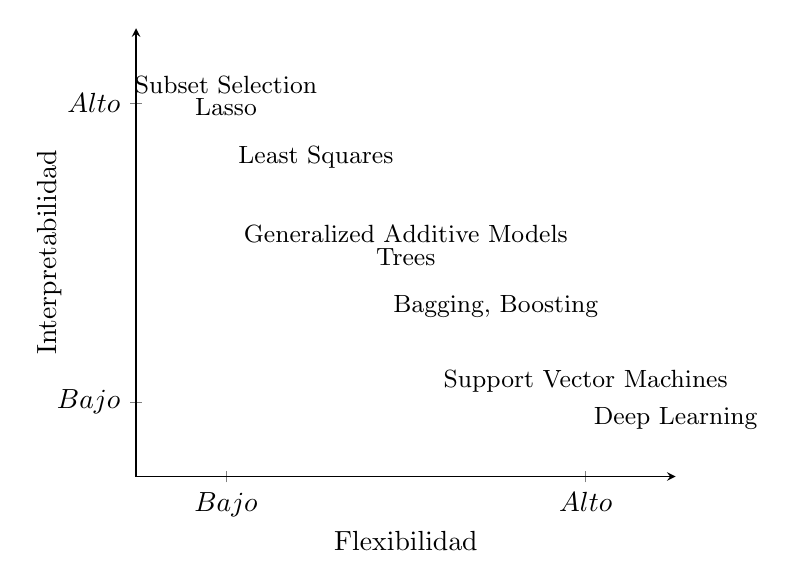
\begin{tikzpicture}
      \begin{axis}[
	xlabel={Flexibilidad},
	ylabel={Interpretabilidad},
	axis lines=middle,
	xmin=0, xmax=6,
	ymin=0, ymax=6,
	xtick={1, 5},
	xticklabels={$Bajo$, $Alto$},
	ytick={1, 5},
	yticklabels={$Bajo$, $Alto$},
	legend style={at={(0.5,-0.3)},anchor=north},
	x label style={at={(axis description cs:0.5,-0.1)},anchor=north},
	y label style={at={(axis description cs:-0.12,0.5)},anchor=south,rotate=90}, % Etiqueta y vertical
	]
	\addplot[only marks, nodes near coords, point meta=explicit symbolic] table[meta=label] {
	    x y label
	    1 5 {\small Subset Selection}
	    1 4.7 {\small Lasso}
	    2 4 {\small Least Squares}
	    3 3 {\small Generalized Additive Models}
	    3 2.7 {\small Trees}
	    4 2 {\small Bagging, Boosting}
	    5 1 {\small Support Vector Machines}
	    6 .5 {\small Deep Learning}
	};
      \end{axis}
    \end{tikzpicture}

    \small Una representación de la compensación entre flexibilidad e interpretabilidad, utilizando diferentes métodos de aprendizaje estadístico. En general, a medida que aumenta la flexibilidad de un método, disminuye su interpretabilidad.
\end{center}

Cuando el objetivo es la inferencia, existen claras ventajas al utilizar métodos de aprendizaje estadístico simples y relativamente inflexibles. Sin embargo, en algunos entornos sólo nos interesa la predicción y la interpretabilidad del modelo predictivo simplemente no es de interés. Por ejemplo, si buscamos desarrollar un algoritmo para predecir el precio de una acción, nuestro único requisito para el algoritmo es que prediga con precisión; la interpretabilidad no es una preocupación. En este contexto, podríamos esperar que sea mejor utilizar el modelo más flexible disponible. Pero este no es siempre el caso. A menudo obtendremos predicciones más precisas utilizando un método menos flexible. Este fenómeno, que puede parecer contradictorio a primera vista, tiene que ver con el potencial de sobreajuste en métodos altamente flexibles. \\

La mayoría de los problemas de aprendizaje estadístico pertenecen a una de estas dos categorías: \textit{supervisados} o \textit{no supervisados}. El aprendizaje supervisado tiene una respuesta asociada $y_i$, contrario al aprendizaje no supervisado. \\

Solemos referirnos a los problemas con una respuesta cuantitativa como problemas de regresión, mientras que los que implican una respuesta cualitativa se suelen denominar problemas de clasificación.\\

\setcounter{section}{1}
\section{Evaluación de la precisión del modelo}
\textbf{\textit{Seleccionar el mejor método puede ser uno de los mayores retos a la hora de llevar a la práctica el aprendizaje estadístico.}}\\

\subsection{Medición de la calidad de ajuste}
Necesitamos cuantificar hasta qué punto el valor de respuesta predicho para una observación dada se aproxima al valor de respuesta verdadero para esa observación. En el ámbito de la regresión, la medida más utilizada es el error cuadrático medio (ECM), dado por
$$MSE=\dfrac{1}{n}\sum_{i=1}^n \left[y_i-\hat{f}\left(x_i\right)\right]^2,$$
donde $\hat{f}\left(x_i\right)$ es la predicción que $\hat{f}$ da para la $i$-ésima observación $x_i$. $MSE$ será pequeño si las respuestas previstas son muy cercanas a las respuestas verdaderas, y serán grandes si para algunas de las observaciones, las respuestas previstas difieren sustancialmente.\\
No nos importa realmente lo bien que funciona el método de entrenamiento con los datos. Más bien, nos interesa la precisión de las predicciones que obtenemos cuando aplicamos nuestro método a datos de prueba no vistos previamente.\\

Queremos elegir el método que ofrezca el MSE de prueba más bajo. Es decir, si tuviéramos un gran número de observaciones de prueba, podríamos calcular
$$Ave\left[y_0-\hat{f}\left(x_0\right)\right]^2,$$
el error cuadrático medio de predicción para estas observaciones de prueba $(x_0,y_0)$. \\

A medida que aumenta la flexibilidad del modelo, el MSE de entrenamiento disminuye, pero no así el MSE de prueba. Cuando un método determinado produce un MSE de entrenamiento pequeño pero un MSE de prueba grande, se dice que estamos sobreajustando los datos. Esto ocurre porque nuestro procedimiento de aprendizaje estadístico está trabajando demasiado para encontrar patrones en los datos de entrenamiento, y puede estar detectando algunos patrones que sólo son causados por el azar en lugar de por las verdaderas propiedades de la función desconocida $f$. Cuando sobreajustamos los datos de entrenamiento, el MSE de prueba será muy grande porque los supuestos patrones que el método encontró en los datos de entrenamiento simplemente no existen en los datos de prueba. Tenga en cuenta que, independientemente de si se ha producido sobreajuste o no, casi siempre esperamos que el MSE de entrenamiento sea menor que el MSE de prueba, porque la mayoría de los métodos de aprendizaje estadístico buscan directa o indirectamente minimizar el MSE de entrenamiento. El sobreajuste se refiere específicamente al caso en el que un modelo menos flexible habría producido un MSE de prueba menor.


\subsection{El sesgo-varianza trade-off}
Es posible demostrar que el $MSE$ esperado de la prueba, para un valor dado $x_0$ siempre puede descomponerse en la suma de tres cantidades fundamentales: La varianza de $\hat{f}\left(x_0\right)$, el sesgo al cuadrado de $\hat{f}\left(x_0\right)$ y la varianza de los términos de error. Esto es,
$$\E\left[y_0-\hat{f}\left(x_0\right)\right]^2 = \Var\left[\hat{f}\left(x_0\right)\right] + \left\{\bias\left[\hat{f}\left(x_0\right)\right]\right\}^2 + \Var\left(\epsilon\right).$$
Aquí la notación $\E\left[y_0-\hat{f}\left(x_0\right)\right]^2$ se define como el MSE esperado de la prueba en $x_0$. Esta ecuación nos dice que para minimizar el error de prueba esperado, tenemos que seleccionar un método de aprendizaje estadístico que consiga simultáneamente una varianza y un sesgo bajos. La varianza se refiere a la cantidad en la que $\hat{f}$ cambiaría si la estimáramos utilizando un conjunto de datos de entrenamiento diferente. Así, que la idea es que la estimación de $f$ no varíe demasiado entre conjuntos de entrenamiento. En general, los métodos estadísticos más flexibles tienen mayor varianza. Por otro lado, el sesgo se refiere al error que se introduce al aproximar un problema de la vida real, que puede ser extremadamente complicado, mediante un modelo mucho más simple. \\
Así, en general, a medida que utilicemos métodos más flexibles, la varianza aumentará y el sesgo disminuirá. La tasa relativa de cambio de estas dos cantidades determinará si el MSE de la prueba aumenta o disminuye. A medida que aumenta, el sesgo tiende a disminuir inicialmente más rápido de lo que aumenta la varianza. En consecuencia, el MSE de prueba disminuye. Sin embargo, llega un momento en el que el aumento de la flexibilidad tiene poco impacto en el sesgo, pero empieza a aumentar significativamente la varianza. Por lo tanto, el MSE de la prueba aumenta. \\

\begin{center}
    \textbf{\textbf{Un buen rendimiento del conjunto de pruebas de un método de aprendizaje estadístico requiere una varianza baja, así como un sesgo al cuadrado bajo. }}\\
\end{center}

 El reto consiste en encontrar un método para el que tanto la varianza como el sesgo al cuadrado sean bajos.

 \subsection{El contexto de la clasificación}
 El enfoque más común para cuantificar la precisión de nuestra estimación $\hat{f}$ es la tasa de error de entrenamiento, la proporción de errores que se cometen si aplicamos nuestra estimación $\hat{f}$ a las observaciones de entrenamiento:
 $$\dfrac{1}{n}\sum_{i=1}^n I\left(y_i\neq \hat{y}_i\right).$$
 Aquí $\hat{y}_i$ es la predicción de la etiqueta de clase para la i-ésima observación utilizando $\hat{f}$. $I\left(y_i\neq \hat{y}_i\right)$ es una variable indicadora igual a $1$ si $yi\neq \hat{y}_i$ y cero si $y_i\neq \hat{y}_i$. Este último nos dice que fue clasificada correctamente por nuestro método. Por lo tanto, la ecuación dada calcula la fracción de clasificaciones incorrectas.\\
 Lo que nos interesará encontrar es la tasa de error de prueba, asociada a observaciones de prueba $(x_0,y_0)$ dada por: 
 $$Ave\left[I\left(y_0\neq \hat{y}_0\right)\right],$$
 donde $\hat{y}_0$ es la predicción de la etiqueta de clase que resulta de aplicar el clasificador a la observación de prueba con el predictor $x_0$.

 \subsubsection{El clasificador de Bayes}
 Es posible demostrar que la tasa de error de prueba se minimiza, en promedio, por un clasificador muy simple que asigna cada observación a la clase más probable. En otras palabras, simplemente deberíamos asignar una observación de prueba con el vector predictor $x_0$ a la clase $j$ para la que
 $$Pr\left(Y=j|X=x_0\right)$$
 es Mayor. En un problema de dos clases en el que sólo hay dos valores de respuesta posibles, digamos la clase 1 o la clase 2, el clasificador de Bayes corresponde a la predicción de la clase uno si $Pr(Y = 1|X = x_0 ) > 0.5$, y de la clase dos en caso contrario. El clasificador de Bayes produce la tasa de error de prueba más baja posible, denominada tasa de error de Bayes. Dado que el clasificador de Bayes siempre elegirá la clase de error de Bayes para la que $Pr\left(Y=j|X=x_0\right)$ sea mayor, la tasa de error será la tasa $1-\max_j Pr\left(Y=j|X=x_0\right)$ en $X=x_0$. En general, la tasa global de error de Bayes viene dada por
 $$1-\E\left[\max_j Pr\left(Y=j|X\right)\right],$$
 La tasa de error de Bayes es análoga al error irreducible, discutido anteriormente.


 \subsubsection{K-vecinos más cercanos}
 Calcular el clasificador de Bayes es imposible. Por lo que podemos utilizar el clasificador de K-vecinos más cercanos. Dado un número entero positivo $K$ y una observación de prueba $x_0$, el clasificador KNN identifica primero los $K$ puntos de los datos de entrenamiento más cercanos a $x_0$, representados por $\mathcal{N}_0$. A continuación estima la probabilidad condicional de la clase de $j$ como la fracción de puntos en $\mathcal{N}_0$ cuyos valores de respuesta son iguales a $j$.
 $$Pr(Y=j|X=x_0)=\dfrac{1}{K}\sum_{i\in \mathcal{N}_0}I\left(y_i=j\right).$$
 Finalmente, KNN clasifica la observación de prueba $x_0$ en la clase con la mayor probabilidad.\\

  A medida que K aumenta, el método se vuelve menos flexible y produce un límite de decisión cercano a la linealidad. Esto corresponde a un clasificador de baja varianza pero alto sesgo. Cuando el límite de decisión es demasiado flexible y encuentra patrones en los datos que no se corresponden con el límite de decisión de Bayes. Esto corresponde a un clasificador que tiene un sesgo bajo pero una varianza muy alta.\\

  Tanto en la configuración de regresión como en la de clasificación, elegir el nivel correcto de flexibilidad es fundamental para el éxito de cualquier método de aprendizaje estadístico. El equilibrio entre sesgo y varianza y la forma de U resultante en el error de prueba pueden hacer que ésta sea una tarea difícil.
